% TODO: intro

\subsection{Markov Chain Monte Carlo}

The goal is now to extract information from the distribution defined by \eqref{eq:part_sum}. Expectation values of observables can be sampled using a Monte Carlo approach. Suppose we sample $n$ triangulations $T^{(i)}$ from \eqref{eq:part_sum}. The expectation value of an observable $f(T)$ can then in theory be obtained from
\begin{equation}
    \lim_{n \to \infty} \frac{1}{n} \sum_{i = 1}^n f(T^{(i)})
    \overset{d}{=}
    \ev{f(T)}
    ,
\end{equation}
where the $d$ above the equality denotes that this is a convergence in distribution. Directly sampling triangulations is not viable. Instead, we use a Markov Chain to explore the space of all possible triangulations. Hence, the label Markov Chain Monte Carlo (MCMC) for our approach.

Sampling from \eqref{eq:part_sum} is not practical. It turns out that $\Omega(N) \sim N! 2^N$. This means that for $\lambda > \ln 2$ large volumes are suppressed so that a typical triangulation will contain only a handful of triangles.
However, when $\lambda < \ln 2$ the partition sum \eqref{eq:part_sum} diverges and the problem is ill-defined.
A solution is to consider only triangulations of a certain fixed volume at a time.
An advantage of this approach is that the desired distribution becomes uniform, since the weight of each triangulation depends only on its volume.
In practice, this can be achieved by using Markov Chain updates that keep the number of triangles fixed.

\subsection{Update rules}
% Should we also include alternative update rules we attempted? And why the don't work? It does show the amount of work and consideration we put into constcuting an effective MCMC simulation, but Im not sure.
\paragraph{Ergodicity}
An important property of a triangulation is how its volume is distributed over different timeslices. It therefore makes sense to choose an update rule that can change the length $\ell(t)$ at some time $t$. However, because we wish to fix the volume this change in length should be compensated elsewhere. Thus, we choose a move that takes an edge and accompanying triangles (we refer to such objects as "shards") from some source location, and moves it to some destination. This "shard move" is shown schematically in Fig. \ref{fig:shard_move}. However, this move alone is not enough to be able to reach all possible triangulations. Thus, we introduce another move that can flip the diagonal between two triangles. This "flip move" is shown schematically in Fig. \ref{fig:flip_move}. According to \cite{2012}, this combination of update rules is ergodic.

\begin{figure}
    \centering
    \begin{tikzpicture}

        % initial state for source
        % timeslices
        \draw (0, 0) -- (4, 0);
        \draw (0, 1) -- (4, 1);
        \draw (0, 2) -- (4, 2);

        % timelike connections
        \draw (0, 0) -- (1, 1) -- (0, 2);
        \draw (2, 0) -- (1, 1) -- (2, 2);
        \draw (2, 0) -- (3, 1) -- (2, 2);
        \draw (4, 0) -- (3, 1) -- (4, 2);

        % shard
        \draw[triangle = {red}] (2, 0) -- (3, 1) -- (2, 1) -- cycle;
        \draw[triangle = {red}] (2, 1) -- (3, 1) -- (2, 2) -- cycle;

        % order 4 vertex
        \node[order4] at (2, 1){};

        % initial state for destination
        % timeslices
        \draw (0, 3) -- (4, 3);
        \draw (0, 4) -- (4, 4);
        \draw (0, 5) -- (4, 5);

        % timelike connections
        \draw (0, 3) -- (1, 4) -- (0, 5);
        \draw (2, 3) -- (1, 4) -- (2, 5);
        \draw (2, 3) -- (3, 4) -- (2, 5);
        \draw (4, 3) -- (3, 4) -- (4, 5);

        % crack
        \draw[edge = {blue}] (2, 3) -- (3, 4) -- (2, 5);

        % final state for source
        % timeslices
        \draw (6, 0) -- (10, 0);
        \draw (6, 1) -- (10, 1);
        \draw (6, 2) -- (10, 2);

        % timelike connections
        \draw (6, 0) -- (7, 1) -- (6, 2);
        \draw (8, 0) -- (7, 1) -- (8, 2);
        \draw (8, 0) -- (9, 1) -- (8, 2);
        \draw (10, 0) -- (9, 1) -- (10, 2);

        % crack
        \draw[edge = {red}] (8, 0) -- (9, 1) -- (8, 2);

        % final state for destination
        % timeslices
        \draw (6, 3) -- (10, 3);
        \draw (6, 4) -- (10, 4);
        \draw (6, 5) -- (10, 5);

        % timelike connections
        \draw (6, 3) -- (7, 4) -- (6, 5);
        \draw (8, 3) -- (7, 4) -- (8, 5);
        \draw (8, 3) -- (9, 4) -- (8, 5);
        \draw (10, 3) -- (9, 4) -- (10, 5);

        % shard
        \draw[triangle = {blue}] (8, 3) -- (9, 4) -- (8, 4) -- cycle;
        \draw[triangle = {blue}] (8, 4) -- (9, 4) -- (8, 5) -- cycle;

        % order 4 vertex
        \node[order4] at (8, 4){};

        % arrow
        \draw[->, ultra thick] (4.5, 2.5) -- (5.5, 2.5);

    \end{tikzpicture}
    \caption{Shard move update rule. Shard source in red (bottom), destination in blue (top). Initial (left) and final (right) states. Order 4 vertices affected by this move are marked with a green dot.}
    \label{fig:shard_move}
\end{figure}

\begin{figure}
    \centering
    \begin{tikzpicture}
        % initial state
        % timeslices
        \draw (0, 0) -- (3, 0);
        \draw (0, 1) -- (3, 1);

        % timelijke connections
        \draw (1, 0) -- (0, 1);
        \draw (1, 0) -- (1, 1);
        \draw (2, 0) -- (2, 1);
        \draw (2, 0) -- (3, 1);

        % diagonal
        \draw[edge = {blue}] (1, 0) -- (2, 1);

        % maybe order 4 vertices
        \node[maybe_order4] at (1, 1){};
        \node[maybe_order4] at (2, 0){};

        % final state
        % timeslices
        \draw (5, 0) -- (8, 0);
        \draw (5, 1) -- (8, 1);

        % timelijke connections
        \draw (6, 0) -- (5, 1);
        \draw (6, 0) -- (6, 1);
        \draw (7, 0) -- (7, 1);
        \draw (7, 0) -- (8, 1);

        % diagonal
        \draw[edge = {blue}] (6, 1) -- (7, 0);

        % maybe order 4 vertices
        \node[maybe_order4] at (6, 0){};
        \node[maybe_order4] at (7, 1){};

        % arrow
        \draw[<->, ultra thick] (3.5, 0.5) -- (4.5, 0.5);
    \end{tikzpicture}
    \caption{Flip move update rule. The flipped edge is shown in blue. Order 4 vertices (if they exist) are marked with a green circle.}
    \label{fig:flip_move}
\end{figure}

\paragraph{Detailed Balance}
But this is not the whole story. Using these update rules we can now sample all triangulations of a given volume, but can we do so \emph{uniformly}, as required by \eqref{eq:part_sum}? A common way to ensure this is to enforce detailed balance. Since in this case the desired distribution is uniform, this amounts to enforcing
\begin{equation}
    p(T \to T') = p(T' \to T),
\end{equation}
for any two triangulations $T$ and $T'$. Here $p(T \to T')$ is the probability to go from $T$ to $T'$ in a single Markov Chain step.

First consider the shard move. In order to be able to remove a shard, we need a vertex of order 4 (i.e.: a vertex with 4 edges)\footnote{If you are worried that such a vertex might not always exist, you are correct. However, if this is the case we can simply perform the flip move instead.}. Start by uniformly choosing such a vertex. To be consistent, we always remove the shard to the right of the selected vertex. Then we uniformly choose a spacelike edge (which is not the edge in the shard) and insert the shard to the left of it. This is done in such a way that an order 4 vertex is created between the selected and inserted edges (see Fig. \ref{fig:shard_move}). The probability of performing a particular instance of this move is then\footnote{Note that here $T$ and $T'$ must be two triangulations that are related by a single application of a shard move. If they are not, the probabilities vanish in both directions and detailed balance is satisfied automatically.}
\begin{equation}
    p_{\text{shard}}(T \to T') = \frac{1}{V_4 (N/2 - 1)},
\end{equation}
with $V_4$ the number of order 4 vertices, and $N$ the number of triangles. Note that this move preserves $V_4$: One order 4 vertex is always destroyed where the shard is taken, and one is always created where it is inserted. Any surrounding vertices are not affected. Since $N$ is also constant, the inverse move will have identical probability and detailed balance is satisfied.

Now consider the flip move. This move is possible where neighbouring triangles have opposite orientation. First uniformly choose a triangle. To be definite, consider its neighbour to the right. If these two triangles have opposite orientation, perform the flip. If this is not the case, reject the move but still count it as a step in the Markov Chain. The probability of performing a particular instance of this move
\begin{equation}
    p_{\text{flip}}(T \to T') = \frac{1}{N}.
\end{equation}
Because $N$ is fixed it is clear that this move obeys detailed balance. Note that since both these moves independently satisfy detailed balance, they can be performed in any sequence. See section \ref{sec:implementation} for more details on how these two moves are combined.

\subsection{Implementation}\label{sec:implementation}
% This was probably the most substantional amount of work of this project, so I think this should be reflected in the size of this part
% Also here I'm not sure whether to include the failed attempts?

\paragraph{Data Structures}
% triangles have local information -> faster markov chain
% order 4 list
How can one actually represent a triangulation inside a computer? There are of course multiple ways to approach this. By far the most frequent operation in the model is performing Markov Chain steps. It therefore makes sense to choose a data structure in which it is easy (i.e. fast) to execute these steps. To facilitate this, we choose to store only adjacency information. Because of this, the computation time of executing a Markov Chain step is constant, and does not scale with the system size. However, the computation time of doing measurements does scale linearly with $N$. But this is not so bad, since measurements are only performed in a fraction of all Markov Chain steps.

In particular, we keep a list of all \verb|triangles|. Then for each \verb|Triangle| we store three labels corresponding to each of their neighbours (neighbours to the \verb|left|, \verb|right| and in the \verb|time|like directions), as well as its \verb|Orientation| (whether it points \verb|Up| or \verb|Down|). Finally, for quick access a list of \verb|order_four| vertices is stored (labelled by the \verb|Triangle| northwest of the vertex). All of this information is stored in the \verb|Universe| structure. In pseudocode the \verb|Universe| is defined as:
\begin{verbatim}
    Universe = {
        triangles: [Triangle],
        order_four: [int],
    }
\end{verbatim}
And the \verb|Triangle| structure is defined as (in pseudocode):
\begin{verbatim}
    Triangle = {
        orientation: Orientation,
        time: int,
        left: int,
        right: int,
    }
\end{verbatim}
Note that we use \verb|int|egers to label \verb|Triangle|s by index in the list of \verb|triangles| stored in \verb|Universe|.

With these data structures the implementation of the moves is relatively straightforward. Uniformly sampling a \verb|triangle| or \verb|order_four| vertex can be done by simply generating a random \verb|int|eger between $1$ and the length of \verb|triangles| or \verb|order_four|, respectively. Sampling a spacelike edge is achieved by sampling a \verb|triangle| and selecting its spacelike edge.

In order to actually execute the shard move, six pairs of neighbours need to be reassigned, and a single \verb|order_four| vertex is moved\footnote{If the order 4 vertices were labelled by the triangles northeast of them, even this would not be necessary. In that case the order 4 vertex would automatically move with the shard to its new location. Unfortunately we only realised this near the very end of the project.}. For the flip move, two pairs of neighbours need to be updated. There are two vertices that might become \verb|order_four|. Additionally, there are two that, if they were \verb|order_four| before the move, they certainly no longer are afterwards. These four vertices are marked with green circles in Fig. \ref{fig:flip_move}, and they should be checked explicitly.

\paragraph{Length Measurements}
% Explain how length profile is measured
So far we have focussed on how the update rules are implemented. However, another very important aspect of the simulation is doing measurements. Perhaps the most obvious thing one can measure on a triangulation is the volume of each timeslice. In our case, each timeslice is a one-dimensional ring, so its volume (or length) can be described by the number of edges (or equivalently the number of vertices) it consists of. Doing this for every timeslice $t$ results in a \emph{length profile} $\ell(t)$. All other observables considered in this work are derived from $\ell(t)$, see section \ref{sec:observables} for more details.

But how can this measurement be performed on our \verb|Universe|? First we choose (it does not really matter how) a \verb|Triangle| to use as reference. We keep walking to the \verb|right| until we reach the original \verb|Triangle| again. The amount of \verb|Up|ward pointing \verb|Triangle|s we passed is then the length $\ell(0)$ of the first timeslice, specifically of the lower boundary timeslice as we count length by the amount of spacelike edges. We can then move to the next timeslice by going to the \verb|time|like neighbour of a \verb|Down|ward pointing \verb|Triangle|. This is repeated until we encounter the first \verb|Triangle| again.

\paragraph{Visualisation}
Besides being able to inspect the length profile, it is also interesting to be able to visually inspect the triangulation directly.
To be able to do this we recreate the triangles from vertices with coordinates to create a mesh which can then be encoded in a standard computer graphics mesh format or directly rendered by \textsc{Wolfram Mathematica} as we did.

To do this, a list of vertices needs to be created which are linked to the triangles they form the corners of.
This is done similarly to the length profile measurements.
We start at a \verb|Triangle|, label all three vertices and store the triplet of the vertices making up the triangles in clockwise fashion.
Using \verb|right| we go to the next \verb|Triangle|, label the new vertex which is part of this triangle and store the triplet of vertices making sure that the vertices which are already labelled do not get relabelled.
This is repeated until we walk back to the original triangle of this timeslice, making sure that the last \verb|Triangle| in the timeslice introduces no new label as all three vertices have already been labelled.
Then we move to the next timeslice by using a \verb|time|like neighbour of a \verb|Down|ward pointing, and repeat the process.
Note that for the layers after the first the bottom vertices have already been labelled, so one need to make sure these do not get relabelled.
This is repeated until the last timeslice before one is back in the original timeslice.
Then we chose to use a cylindrical visualisation, which makes a cut in the real toroidal topology of the triangulation. So instead of linking the vertices of the first and last timeslice, we simply give the lower vertices of the first timeslice and upper vertices of the last timeslice different labels.
One can create all triangles making up to full toroidal topology without creating a cut, but then one need to be really careful to make sure the labels of the upper vertices of the last timeslice correspond to the correct vertices.

After the list of vertex labels and the triplets of these labels have been created, the coordinates of the vertices need to be determined also called choosing the \emph{embedding}.
We choose a timeslice preserving cylindrical embedding, where the vertices of a timeslice are equally spread around a circle with a circumference reflecting the length of that timeslice and subsequent timeslices are placed parallel to one other a corresponding distance away.
This has the result that all spacelike edges are roughly the same length as one other and as the distance between timeslices. The relative rotation of the timeslices is chosen such that one of the timelike edges has the shortest distance possible between the timeslices; an alternative choice of rotation is to choose it such that the average length of the timelike edges is minimal.
Using this method we can produce visualisations of the triangulations like the one
displayed in Fig. \ref{fig:triangulation_visualisation}.

\begin{figure}[h]
    \centering
    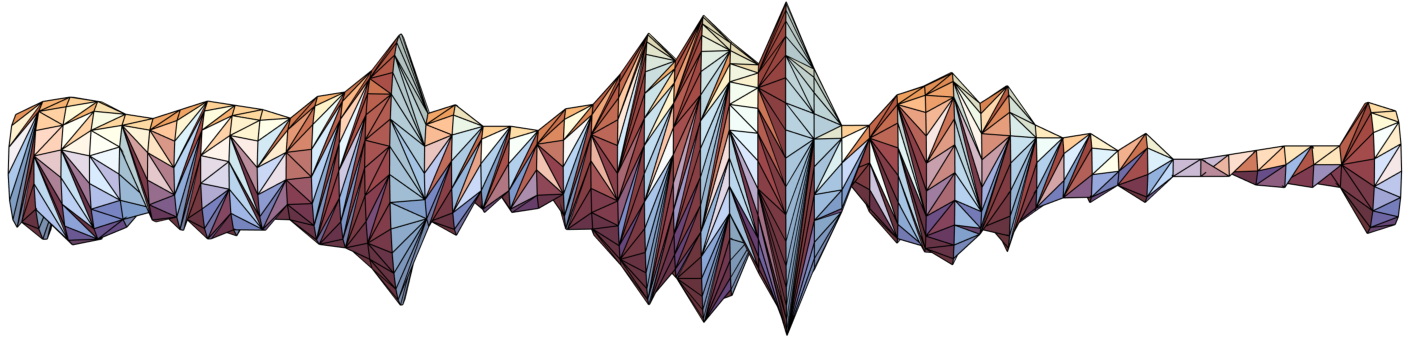
\includegraphics[width=0.98\linewidth]{img/triangulation_visualisation.pdf}
    \caption{A visualisation of a small triangulation using a timeslice preserving cylindrical embedding}
    \label{fig:triangulation_visualisation}
\end{figure}

\paragraph{Command-line Interface}
% explain all relevant input parameters of the cli
In order to actually run a simulation, we of course need to provide some concrete parameter values. The most obvious ones are related to the system size. The number of triangles is fixed, so that would seem like a logical input parameter. However, instead we choose to provide the number of timeslices $T$ and the initial length per timeslice $L$ as input. The total number of triangles is then $N = 2 T L$. This makes it easier to change $T$ and $L$ independently of each other.

Another input parameter has to do with the fact that we are using two different types of Markov Chain moves. We need some way of choosing between these two moves. Therefore, we introduce a move rate $r$. In particular $r$ is the probability that any given move will be a shard move. Note that introducing this rate $r$ does not affect detailed balance: we simply multiply both sides of the detailed balance equation by $r$ (for the shard move) or $1 - r$ (for the flip move). This move ratio can be set separately for the equilibration phase and the measurement phase.

Finally, there are some parameters that are related to the Monte Carlo measurements. The obvious one is of course which observable is measured: the whole length profile $\ell(t)$ or only its standard deviation $\sigma_\ell$. Other parameters include the number of measurements to take, the number of sweeps\footnote{A sweep is defined as $2 T L$ Markov Chain steps.} in-between measurements, the length of the equilibration phase and a path to which the data is written.



\subsection{Observables} \label{sec:observables}
% Explain choice of observables, possibly alternatives that were considered but not measured
% Maybe also explain how lengthprofile is obtained from implementation, as this is not entirely trivial and Timothy asked about this after the presentation
Finding good observables to measure is quite challenging in (C)DT. This may partly be due to a lack of experimental data to compare simulations to.
But also where many Monte Carlo simulations in physics are concerned with describing the behaviour of fields on a lattice, naturally giving some combination of the field values as observables,
there is no such field in CDT but the lattice itself should provide the information of interest.

The chosen observables can of course not depend on any details of the implementation, like the use of labelling in our implementation.
And for an observable to be of physical interest it should also have a well-defined limit for the amount of triangles $N \rightarrow \infty$.
Observables that are often looked at are different notions of dimension, notably the \emph{spectral dimension} \cite{2012} and \emph{Hausdorff dimension} \cite{1998, 2012}, the latter of which has also been discussed in the case of Dynamical Triangulation in the course Monte Carlo Techniques. And a newer observable of interest is a certain notion of \emph{Quantum Curvature} -- a sort of extended notion of Ricci curvature which can be applied to the used triangulations and obeys a proper limit \cite{brunekreef2021}.

However since the focus of this project was more in the implementation of a Markov Chain Monte Carlo simulation, and the measurements and analysis of these observables is somewhat involved, we only consider observables that are derived from the volume of the space-like slices.
This means that in $1 + 1$D CDT we look at the \emph{length}, that is the amount of edges or equivalently the amount of vertices in a time-slice, at different times; this we call the \emph{length profile} $\ell(t)$

\paragraph{Length profile}
The length profile itself still depends on a certain choice of origin in $t$, while we consider a toroidal topology so any there is no preferred origin. Thus, any observable should have some sort of averaging over $t$.

The simplest observable to consider is the average of $\ell(t)$, but this is trivially $L$ since the total amount timeslices and triangles and thus vertices is kept fixed.
So the simplest non-trivial observable we can think of is the standard deviation $\sigma_\ell$ of the length profile $\ell(t)$:
\begin{equation}\label{eq:std_meas}
    \sigma_\ell^2 = \frac{1}{T} \sum_{t = 1}^{T} \Big(\ell(t) - L\Big)^2,
\end{equation}
using the usual definition of the population variance.

%TODO possibly we want to use a different notion of length correlation
But $\sigma_\ell$ does not contain any information of the relation of lengths between different times $t$.
So an arguably more interesting observable is what we call the \emph{length covariance}:
\begin{equation}\label{eq:cov_meas}
    \rho_\ell(t) = \frac{1}{T} \sum_{t_0 = 1}^{T} \qty(\ell(t_0) - L)\qty(\ell(t_0 + t) - L),
\end{equation}
note that $\rho_\ell(0) = \sigma_\ell^2$.
Important to note is that the length correlation is still a function of $t$ but this $t$ is the time difference between two time-slices, so there is no origin dependence.

Both observables $\sigma_\ell$ and $\rho_\ell(t)$ do diverge for $N \rightarrow \infty$ as they will scale with $N$.
How they will scale is at this point not known, but we hope they will scale in a well-behaved way such that with proper rescaling these observables may have a well-defined limit.